\documentclass[aspectratio=169,10pt]{beamer}
\usetheme{metropolis}
\usepackage[spanish,es-nodecimaldot]{babel}
\usepackage[utf8]{inputenc}
\usepackage{booktabs}
\usepackage{graphicx}
\usepackage{listings}
\usepackage{xcolor}
\usepackage{amsmath}
\usepackage{colortbl}
\usepackage{multirow}
\usepackage{array}

% ── Estilo listings para MATLAB ───────────────────────────────────────────────
\definecolor{matlabgreen}{RGB}{28,172,0}
\definecolor{matlablilas}{RGB}{170,55,241}
\lstset{
  language=Matlab,
  basicstyle=\tiny\ttfamily,
  keywordstyle=\color{blue}\bfseries,
  commentstyle=\color{matlabgreen}\itshape,
  stringstyle=\color{matlablilas},
  numbers=none,
  frame=single,
  breaklines=true,
  backgroundcolor=\color{gray!8},
  xleftmargin=2pt,
  xrightmargin=2pt,
  framexleftmargin=2pt
}

% ── Metadatos ────────────────────────────────────────────────────────────────
\title{Replicaci\'on de Carrillo \& Elizondo (2015/2018)}
\subtitle{SVAR con Restricciones de Exclusi\'on y de Signo --- M\'exico}
\author{Carlos Ramírez}
\institute{ITAM}
\date{Abril 2026}

% =============================================================================
\begin{document}

% ── SLIDE 1: PORTADA ─────────────────────────────────────────────────────────
\maketitle

% ── SLIDE 2: AGENDA ──────────────────────────────────────────────────────────
\begin{frame}{Agenda}
\begin{enumerate}
  \item Procesamiento de datos
  \item Diagn\'osticos estad\'isticos
  \item Estrategias de identificaci\'on
  \item Diferencias y conclusiones
\end{enumerate}
\end{frame}

% =============================================================================
% §1  PROCESAMIENTO DE DATOS
% =============================================================================

% ── SLIDE 3: TABLA DE CAMBIOS ────────────────────────────────────────────────
\begin{frame}{\S1 Cambios en el procesamiento de datos}
\begin{center}
\small
\begin{tabular}{lll}
  \toprule
  \textbf{Dimensi\'on} & \textbf{Paper C\&E} & \textbf{Replicaci\'on} \\
  \midrule
  Per\'iodo muestral    & 2001:01--2014:03 ($T=159$)     & 2001:01--2014:03 ($T=159$)            \\
  TCR bilateral         & 21 socios comerciales           & 49 socios (Banxico)                   \\
  Producto dom\'estico  & Brecha IGAE precalculada        & \'Indice IGAE nivel (INEGI)           \\
  Ajuste estacional     & No especificado                 & X-13ARIMA-SEATS (\texttt{R seasonal}) \\
  Filtro de tendencia   & HP $\lambda=129{,}600$          & HP $\lambda=129{,}600$                \\
  $\hat{\beta}_{lower}$ & $-0.700$                        & $-0.715$                              \\
  \bottomrule
\end{tabular}
\end{center}
\vspace{0.2cm}
\small
El ajuste estacional se aplica a inflaci\'on subyacente, INPP y M2
\emph{antes} de calcular los gaps con filtro HP.
\end{frame}

% ── SLIDE 4: SERIES ORIGINALES ───────────────────────────────────────────────
\begin{frame}{\S1 Series originales con tendencia HP ($\lambda=129{,}600$)}
\begin{center}
  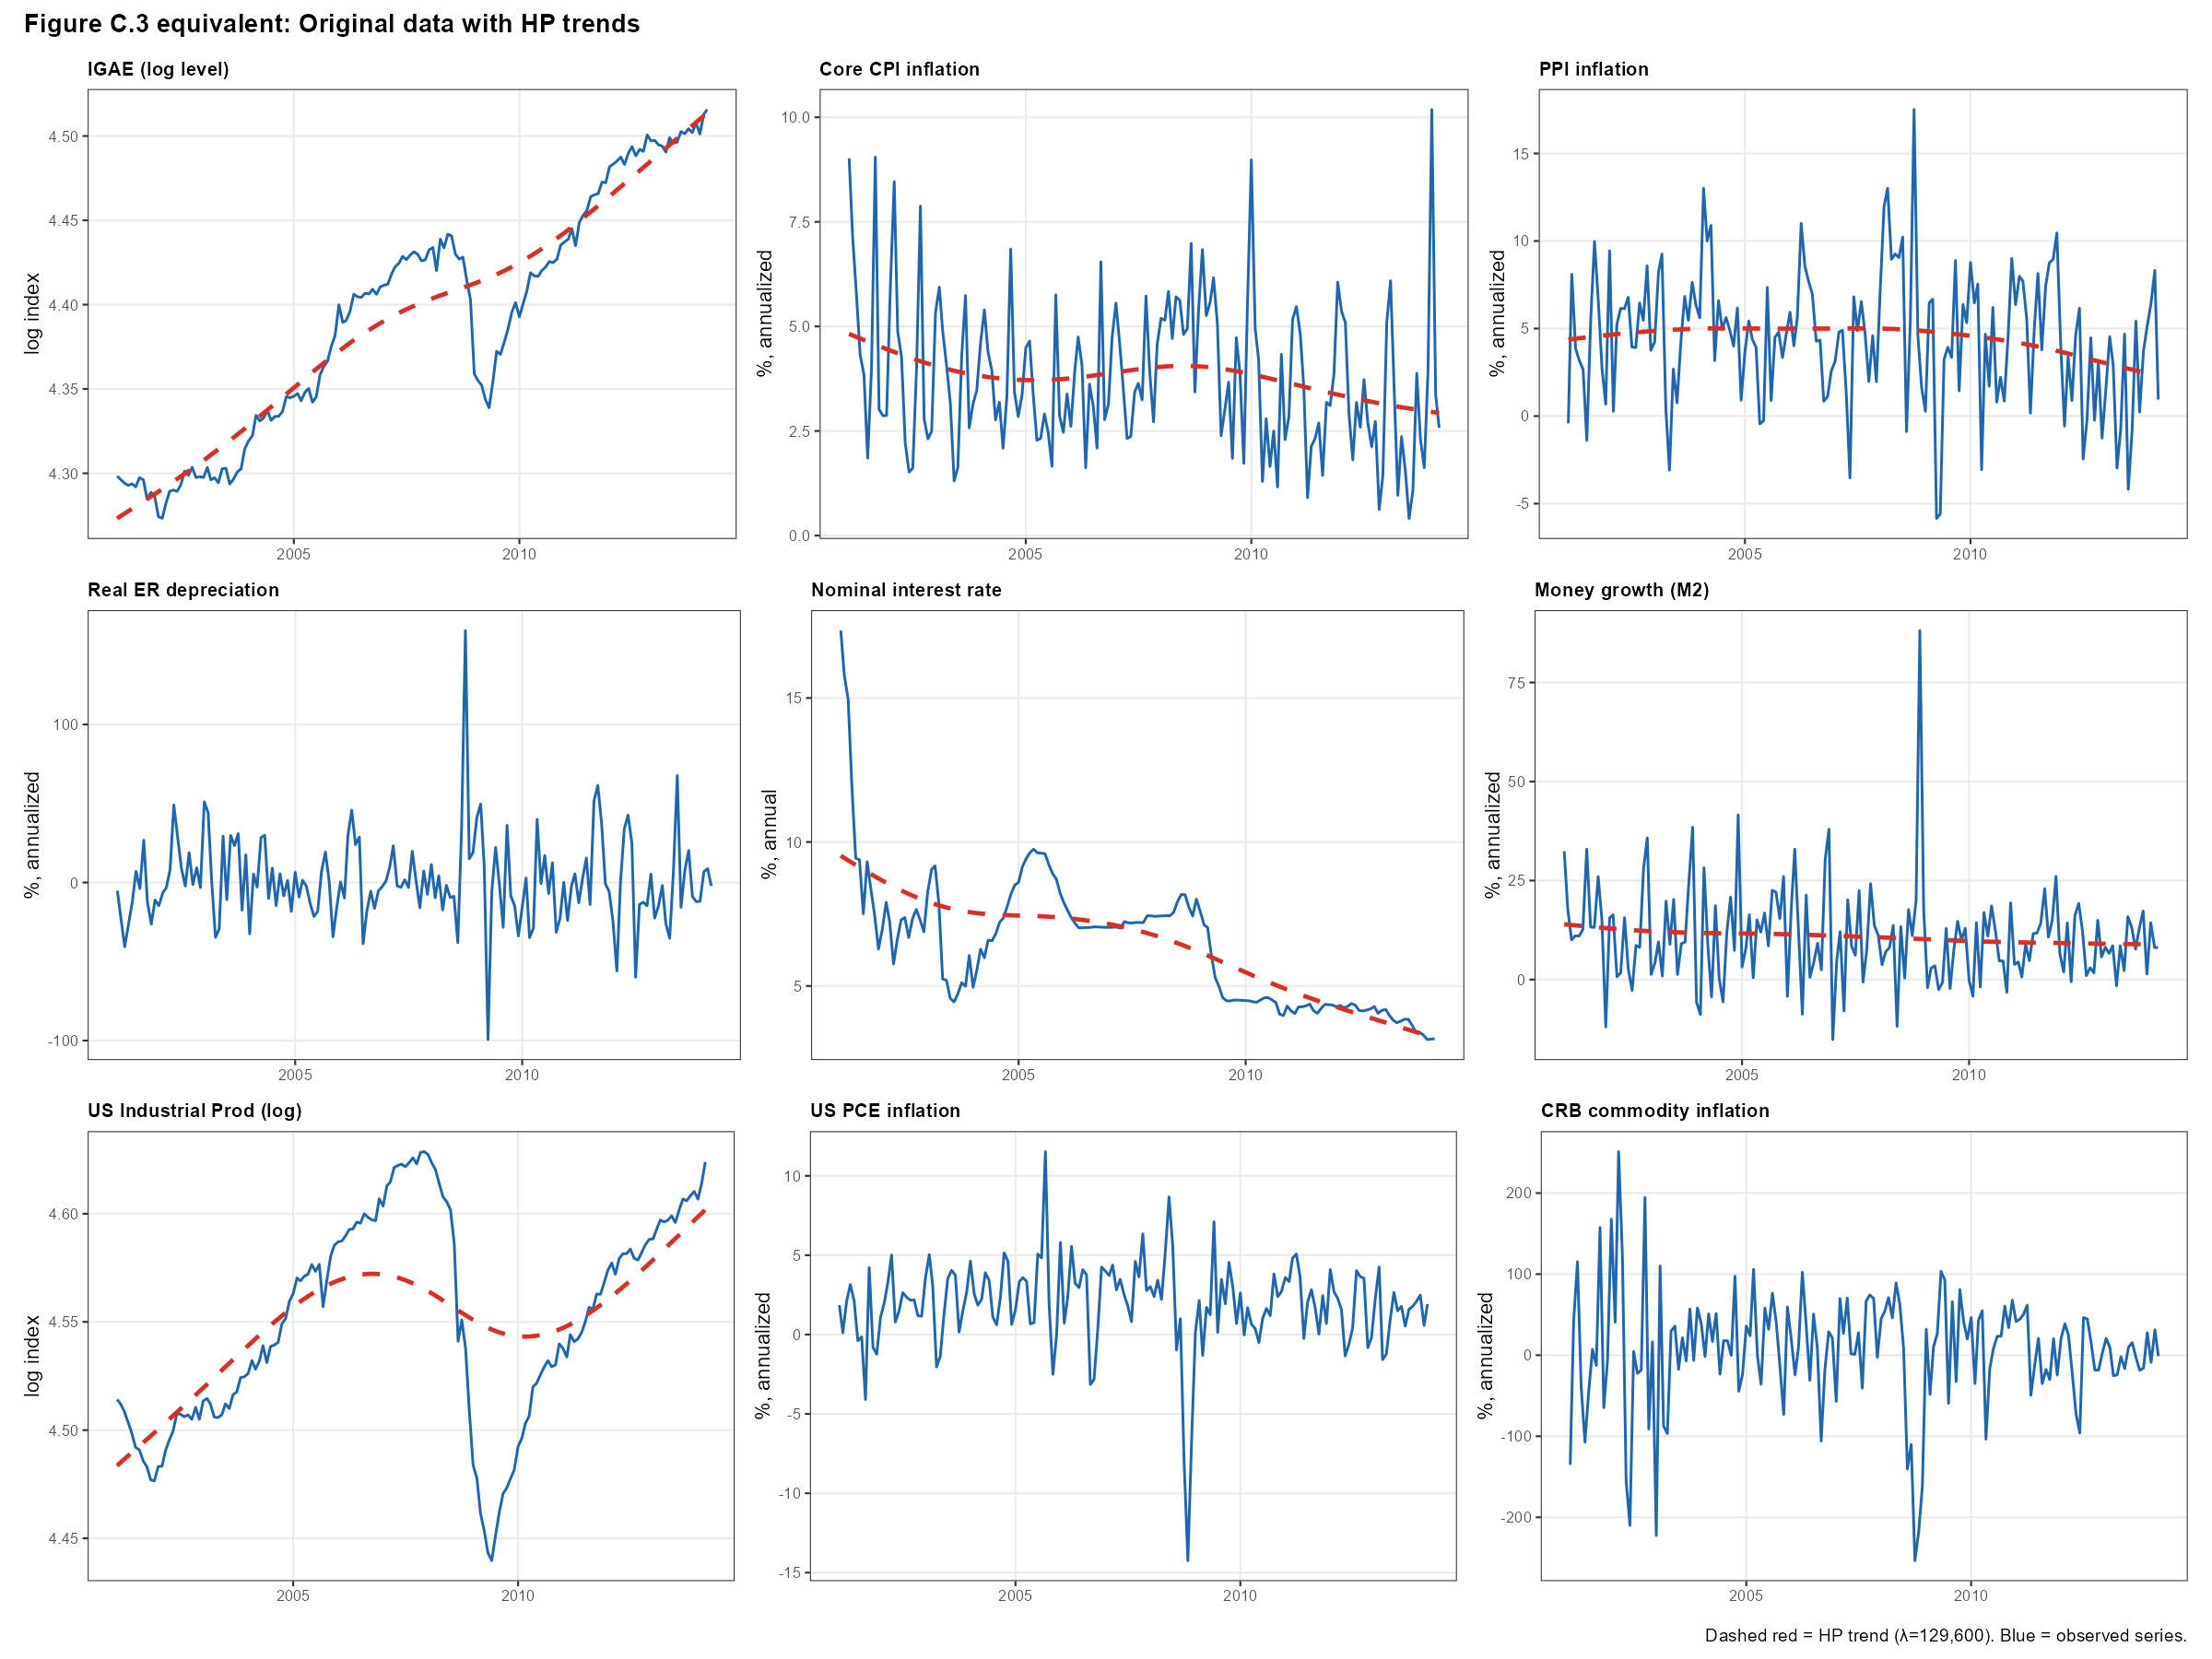
\includegraphics[width=\textwidth,height=0.80\textheight,keepaspectratio]{figures/fig_series_originales.png}
\end{center}
\end{frame}

% ── SLIDE 5: SERIES TRANSFORMADAS ────────────────────────────────────────────
\begin{frame}{\S1 Series transformadas (gaps y tasas anualizadas)}
\begin{center}
  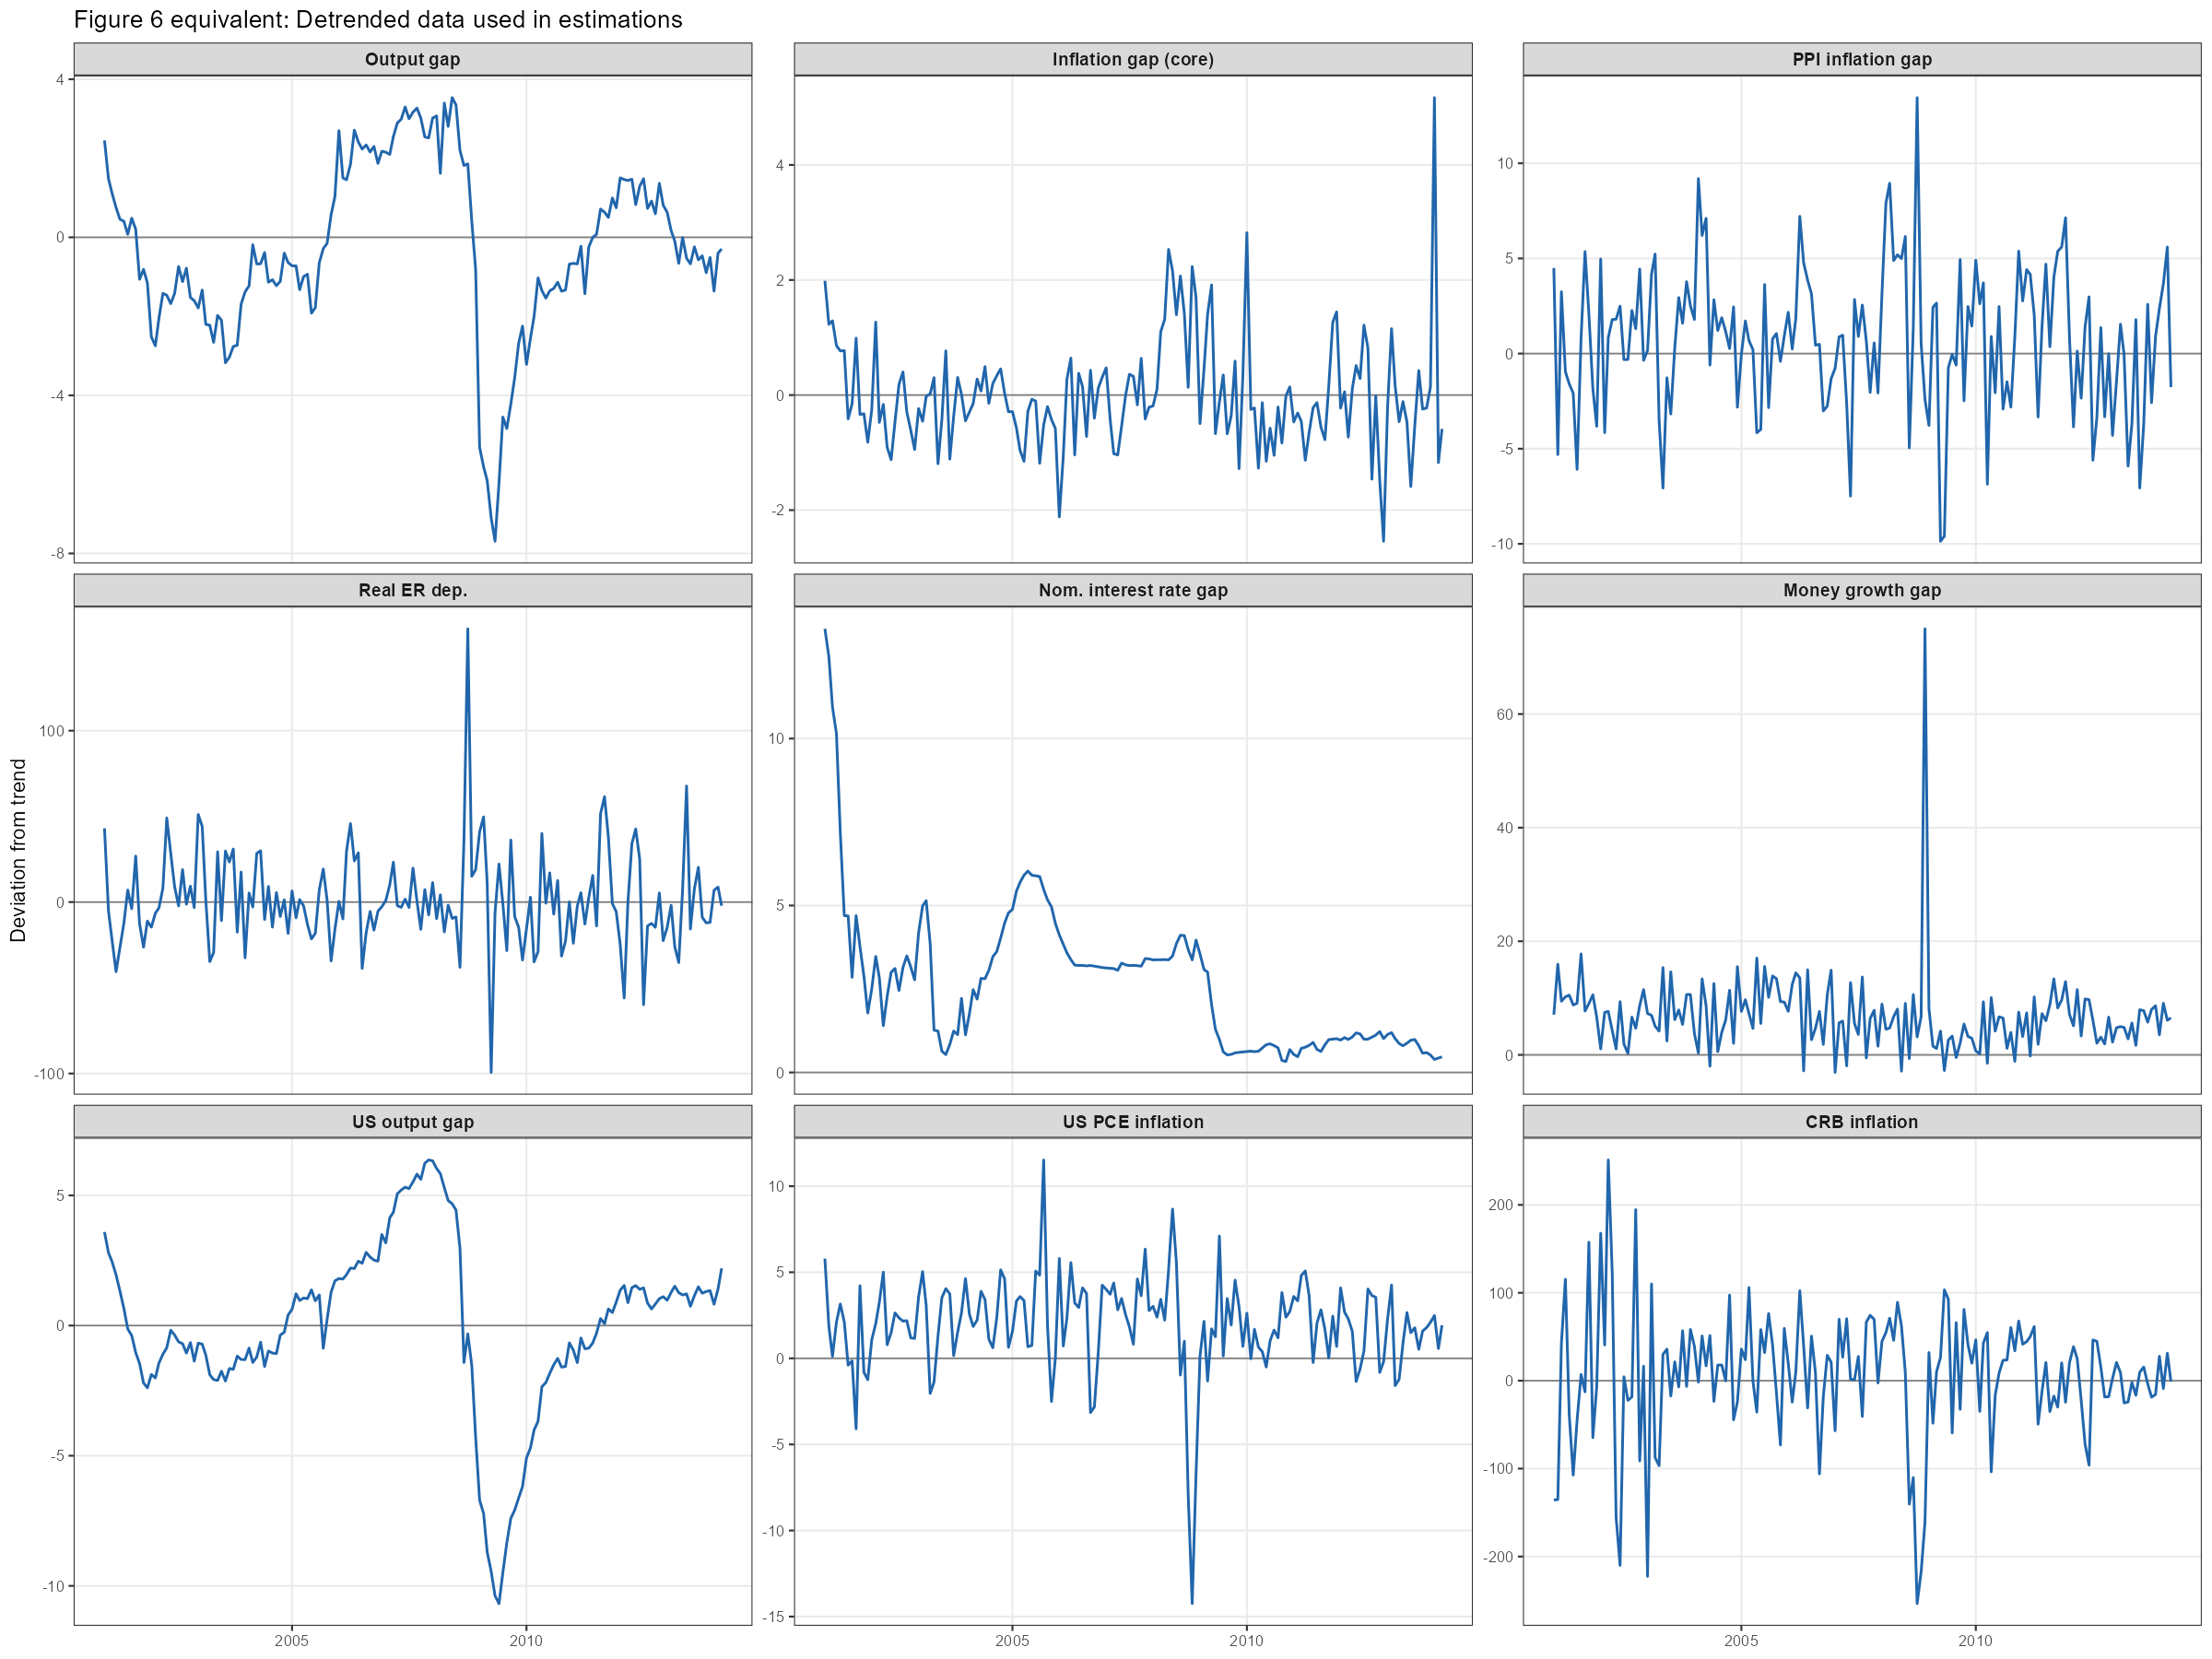
\includegraphics[width=\textwidth,height=0.80\textheight,keepaspectratio]{figures/fig_series_gaps.png}
\end{center}
\end{frame}

% =============================================================================
% §2  DIAGNÓSTICOS
% =============================================================================

% ── SLIDE 6: ADF/PP + REZAGOS + ESTABILIDAD ──────────────────────────────────
\begin{frame}{\S2 Ra\'iz unitaria, selecci\'on de rezagos y estabilidad}
\begin{columns}[T]
\column{0.55\textwidth}
  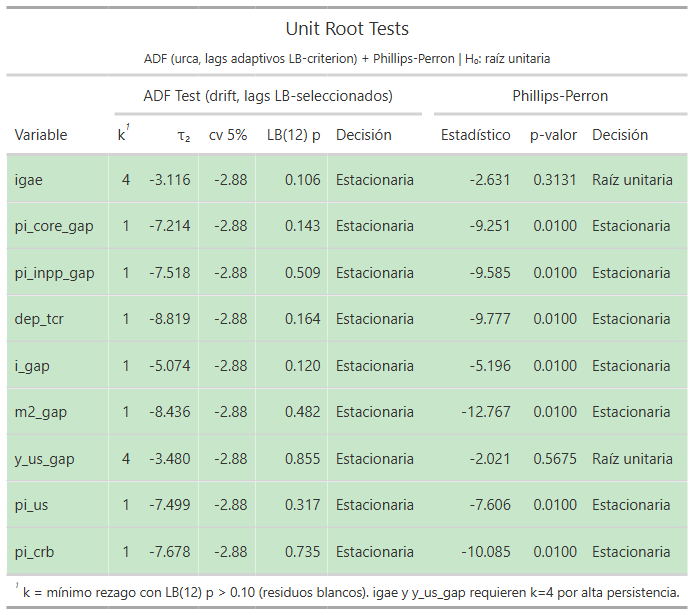
\includegraphics[width=\linewidth,height=0.33\textheight,keepaspectratio]{figures/tabla_adf_pp.png}
  \vspace{0.10cm}
  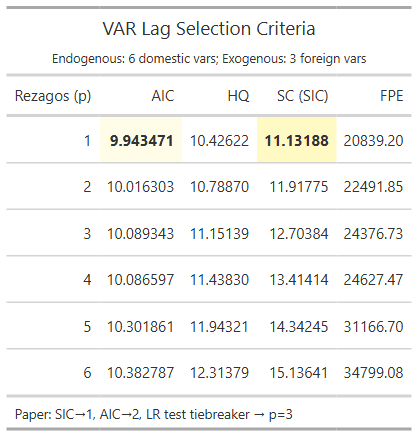
\includegraphics[width=\linewidth,height=0.33\textheight,keepaspectratio]{figures/tabla_varsoc.png}
\column{0.45\textwidth}
  \textbf{Estabilidad del VAR($p=3$):}
  \vspace{0.15cm}
  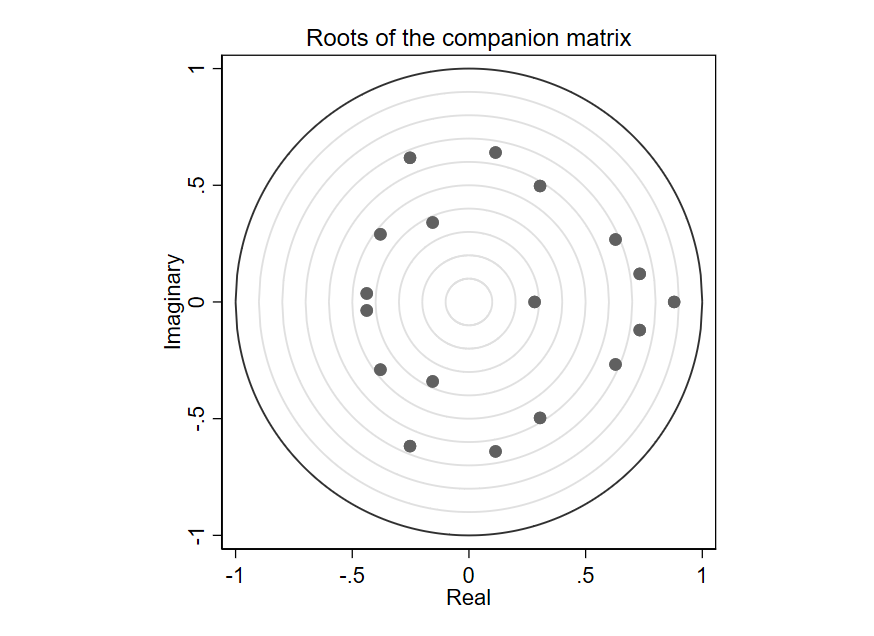
\includegraphics[width=\linewidth,height=0.45\textheight,keepaspectratio]{figures/varstable.png}
  \vspace{0.15cm}
  \small
  \begin{itemize}
    \item ADF/PP: todas las variables $I(0)$ \checkmark
    \item AIC/SIC/LR $\Rightarrow$ $p=3$ \checkmark
    \item Todas las ra\'ices dentro del c\'irculo unitario \checkmark
  \end{itemize}
\end{columns}
\end{frame}

% ── SLIDE 7: AUTOCORRELACIÓN + BETA_LOWER ────────────────────────────────────
\begin{frame}{\S2 Autocorrelaci\'on, normalidad y $\hat{\beta}_{lower}$}
\begin{columns}[T]
\column{0.55\textwidth}
  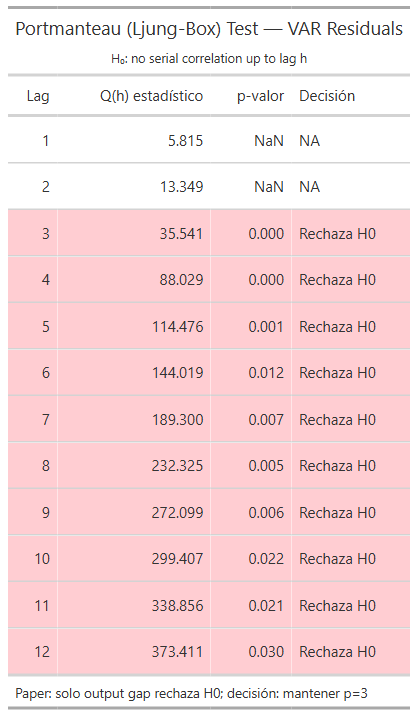
\includegraphics[width=\linewidth,height=0.72\textheight,keepaspectratio]{figures/tabla_lm_norm.png}
\column{0.45\textwidth}
  \textbf{Estimaci\'on de $\hat{\beta}_{lower}$ (Ec.~11):}
  \vspace{0.2cm}
  \begin{block}{}
  \begin{align*}
    \hat{\beta}^-       &= -0.400 \\
    \mathrm{SE}         &= \phantom{-}0.192 \\
    \hat{\beta}_{lower} &= \hat{\beta}^- - 1.645\cdot\mathrm{SE} \\
                        &= -0.715
  \end{align*}
  \end{block}
  \small
  Paper reporta: $\hat{\beta}^-=-0.035$,\;
  $\hat{\beta}_{lower}=-0.7$ \\[4pt]
  \alert{Diferencia en magnitud, misma direcci\'on y orden de magnitud.}
\end{columns}
\end{frame}

% =============================================================================
% §3  ESTRATEGIAS DE IDENTIFICACIÓN
% =============================================================================

% ── SLIDE 8: CHOLESKY (FIGURA 7) ─────────────────────────────────────────────
\begin{frame}{\S3 Estrategia 1: Restricciones de Exclusi\'on (Cholesky)}
\begin{columns}[T]
\column{0.65\textwidth}
  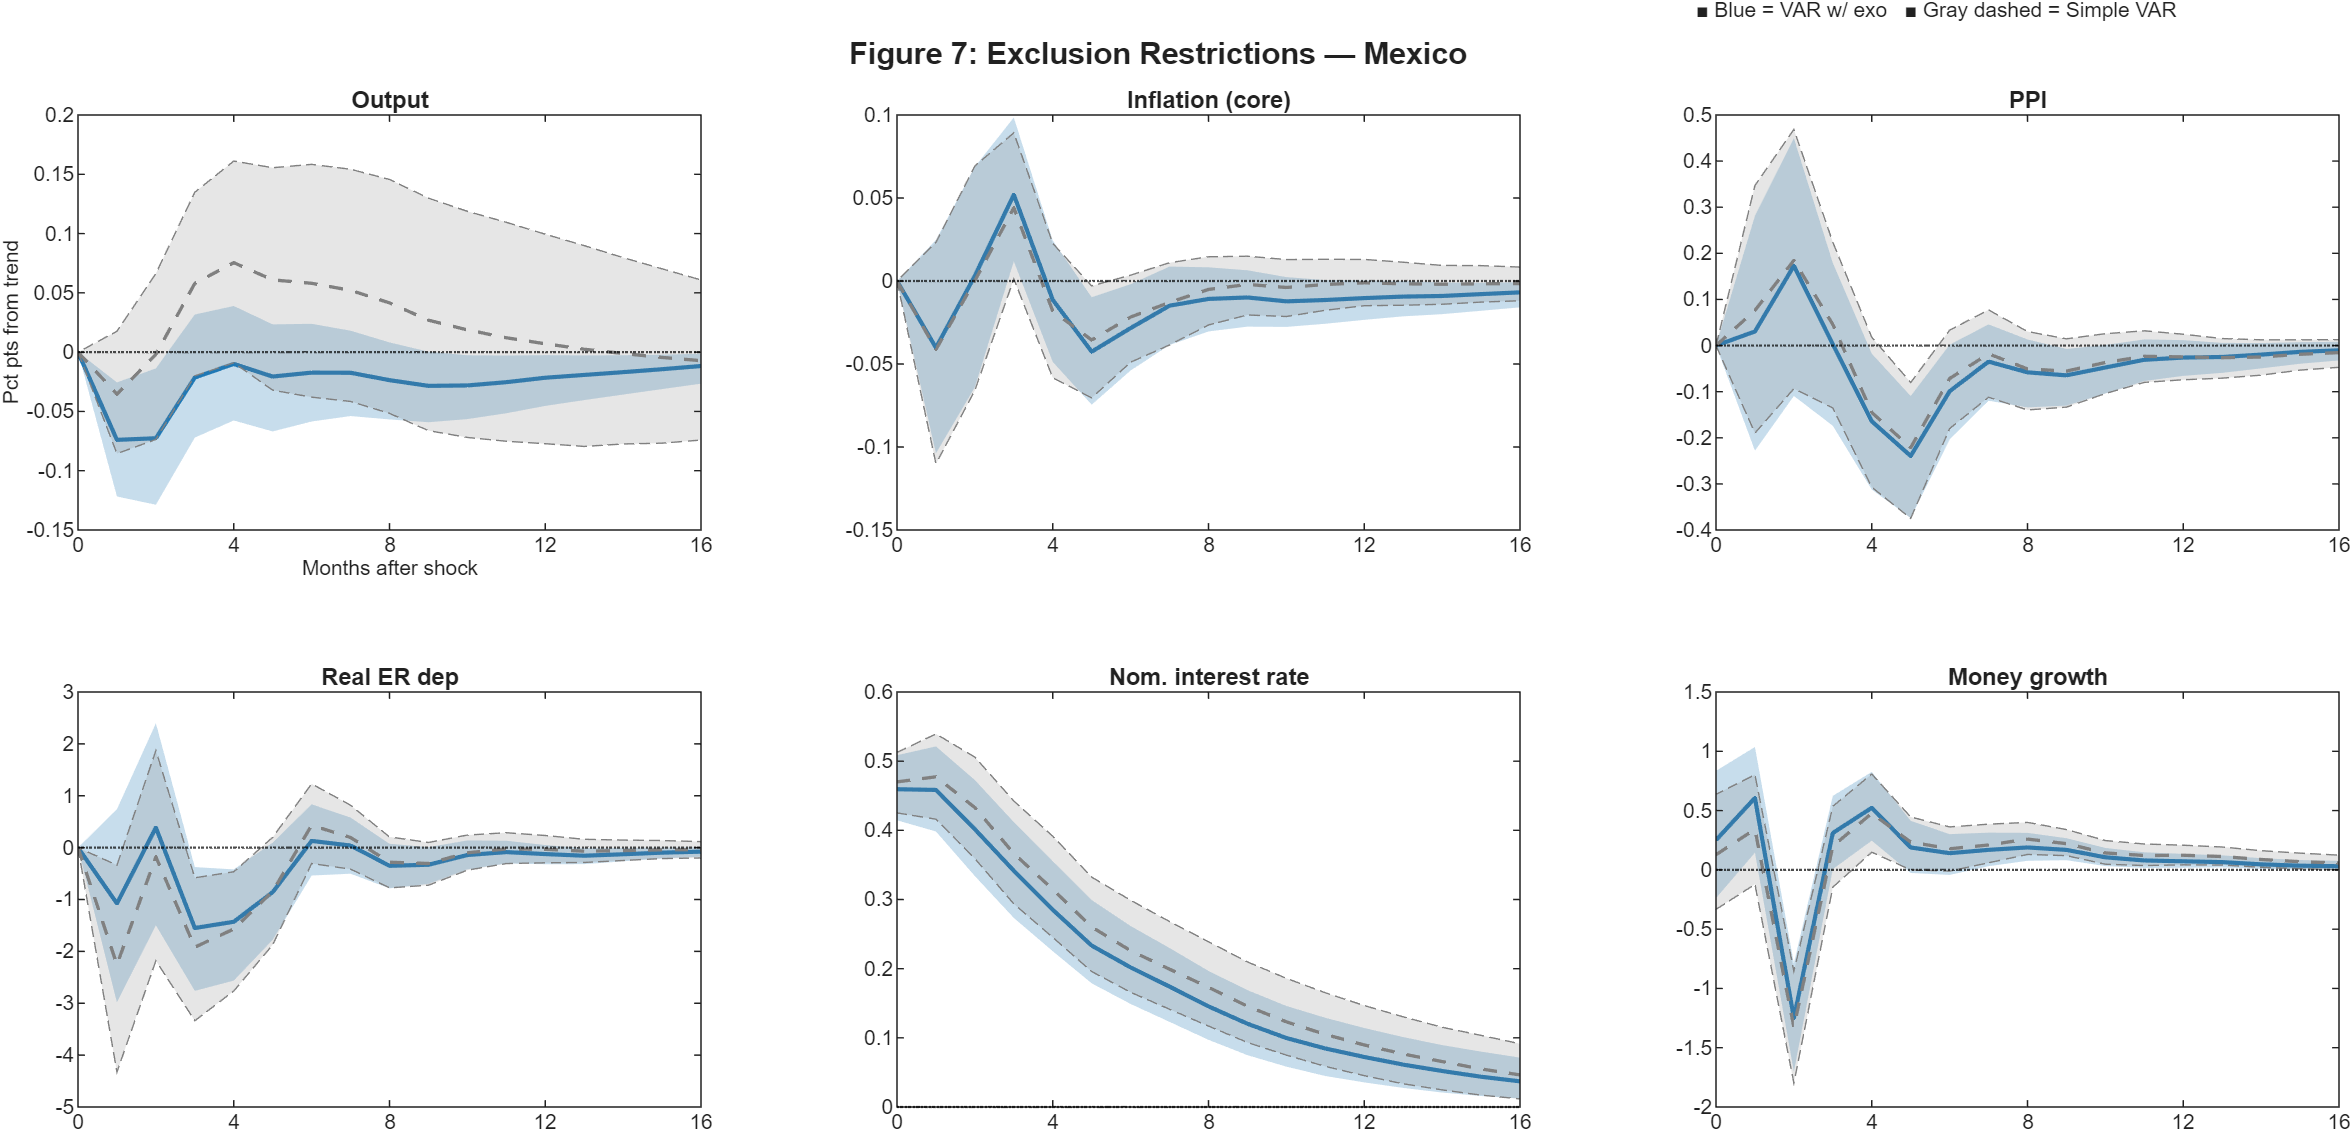
\includegraphics[width=\linewidth,height=0.75\textheight,keepaspectratio]{figures/fig7_exclusion.png}
\column{0.35\textwidth}
  \small
  \textbf{Impactos $h=0$ (choque $+1$\,pp en $i$):}
  \vspace{0.2cm}
  \begin{tabular}{lcc}
    \toprule
    Variable     & Paper      & Rep.     \\
    \midrule
    Output       & $\approx0$ & $0.000$  \\
    $\pi$ core   & $\approx0$ & $0.000$  \\
    PPI          & $\approx0$ & $0.000$  \\
    TCR dep.     & $\approx0$ & $0.000$  \\
    $i$          & $+0.47$    & $+0.466$ \\
    M2           & $+0.31$    & $+0.313$ \\
    \bottomrule
  \end{tabular}
  \vspace{0.2cm}
  \small
  Por construcci\'on del ordenamiento Cholesky,
  las variables 1--4 no reaccionan en $h=0$.
\end{columns}
\end{frame}

% ── SLIDE 9: BOOTSTRAP RUNKLE (CÓDIGO MATLAB) ────────────────────────────────
\begin{frame}[fragile]{\S3 Bootstrap Runkle (1987) --- C\'odigo MATLAB}
\begin{lstlisting}
for b = 1:n_boot
    % 1. Resamplear residuos con reemplazo (Runkle 1987)
    idx    = randi(T_eff, T_eff, 1);
    res_b  = resid0(idx, :);
    % 2. Regenerar pseudo-datos via recursion VAR
    Y_b    = runkle_bootstrap_data(B0, Y, Z, p, res_b, use_exo);
    % 3. Re-estimar VAR -> nueva Sigma_b -> nueva Cholesky P_b
    [B_b, Sig_b, ~, ~] = estimate_var(Y_b, Z, p, use_exo);
    P_b     = chol(Sig_b, 'lower');
    shock_b = P_b(:, j_mp);          % columna del choque monetario
    irf_b   = compute_irf(B_b, n, p, shock_b, h);
    % 4. Acumular IRF del draw
    irfs_boot(b, :, :) = irf_b';
end
% Bandas de confianza al 68% (percentiles 16 y 84)
irf_lo = prctile(irfs_boot, 16, 1);
irf_hi = prctile(irfs_boot, 84, 1);
\end{lstlisting}
\vspace{0.1cm}
\small
\textbf{Clave:} se re-estima $B_0$ \emph{y} $P_b$ en cada r\'eplica
$\Rightarrow$ captura incertidumbre tanto en coeficientes como en la identificaci\'on.
\end{frame}

% ── SLIDE 10: SIGN RESTRICTIONS ESTÁNDAR (FIGURA 8) ─────────────────────────
\begin{frame}{\S3 Estrategia 2: Restricciones de Signo Est\'andar}
\begin{columns}[T]
\column{0.65\textwidth}
  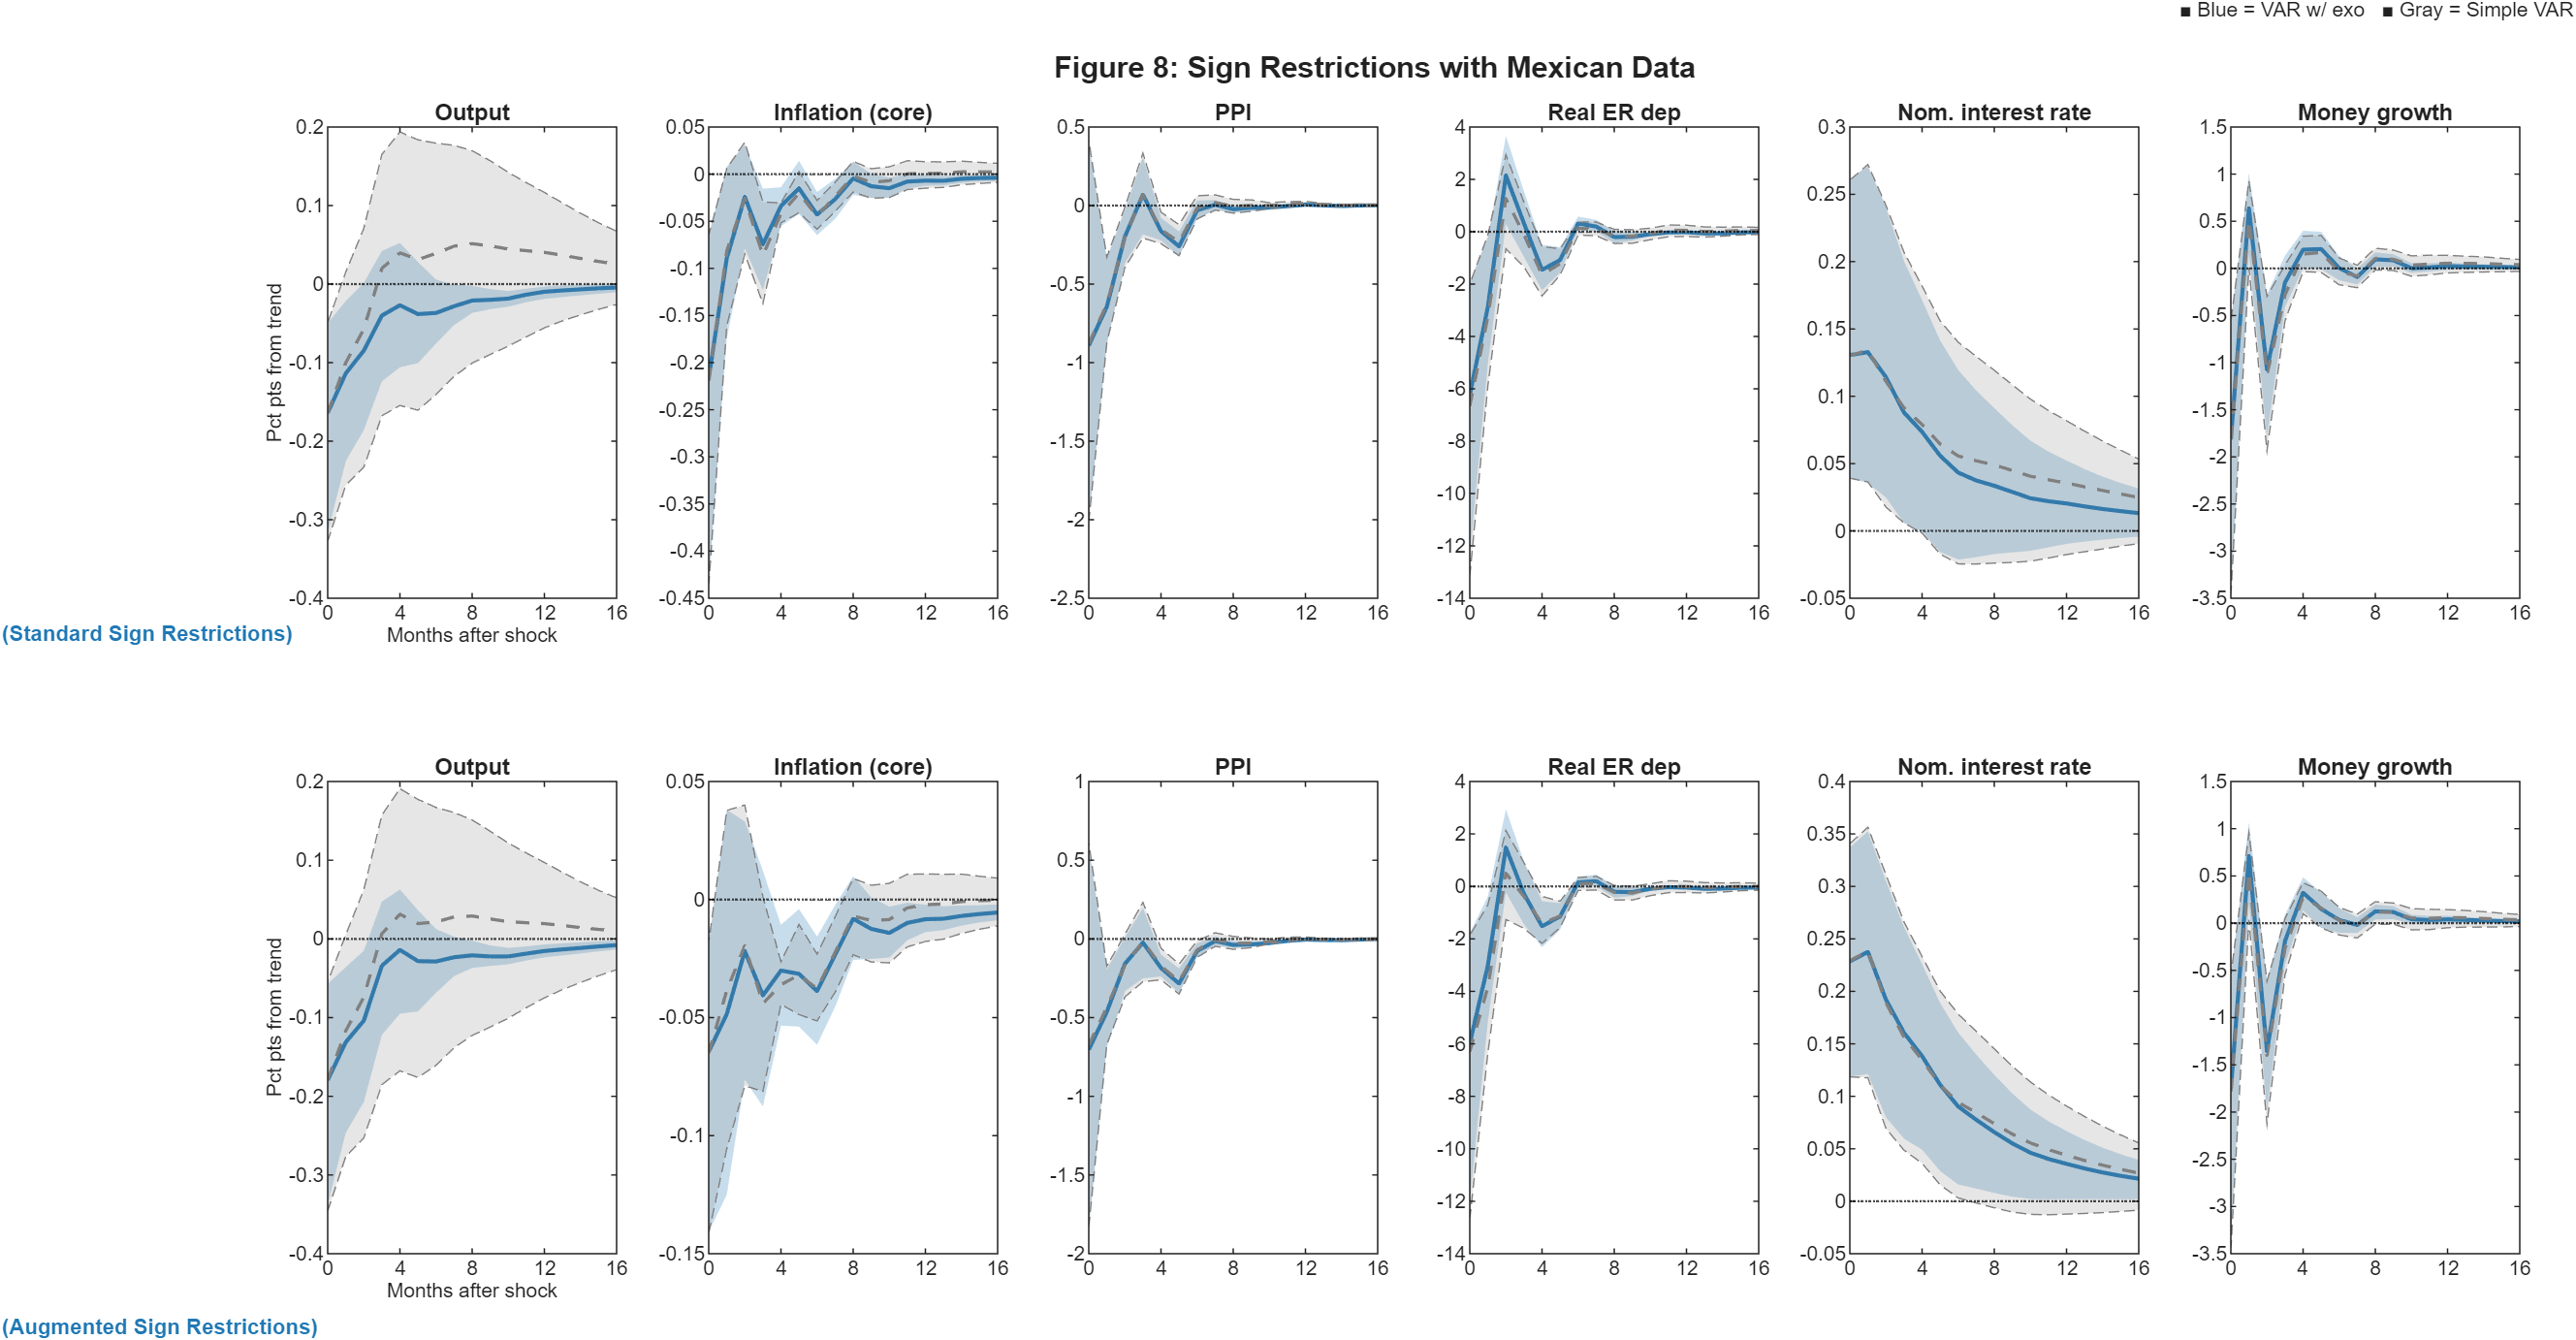
\includegraphics[width=\linewidth,height=0.75\textheight,keepaspectratio]{figures/fig8_sign_restrictions.png}
\column{0.35\textwidth}
  \small
  \textbf{Restricciones al choque monetario (Tabla~2):}
  \vspace{0.2cm}
  \begin{tabular}{lc}
    \toprule
    Variable   & Signo  \\
    \midrule
    Output     & $-$    \\
    $\pi$ core & $-$    \\
    PPI        & libre  \\
    TCR dep.   & $-$    \\
    $i$        & $+$    \\
    M2         & $-$    \\
    \bottomrule
  \end{tabular}
  \vspace{0.25cm}
  \small
  Modelos aceptados:\\
  \textbf{198,654} (est\'andar)\\
  \textbf{66,874} (aumentado)\\[4pt]
  $Q\sim\mathrm{Haar}(n\times n)$,\; $K_{\max}=5{,}000$
\end{columns}
\end{frame}

% ── SLIDE 11: ALGORITMO AUMENTADO (DESCRIPCIÓN) ──────────────────────────────
\begin{frame}{\S3 Algoritmo de Restricciones de Signo Aumentadas}
\textbf{Algorithm~1} (Carrillo \& Elizondo --- adaptaci\'on):
\vspace{0.1cm}
\begin{enumerate}\small
  \item Estimar VAR reducido $\Rightarrow$ $\hat{B}$,\;$\hat{\Sigma}_u$;\;
        calcular $P=\mathrm{chol}(\hat{\Sigma}_u)$
  \item Estimar $\hat{\beta}_{lower}$ (Ec.~11) con Newey--West (3 rezagos)
  \item Para cada draw $b=1,\ldots,B$:
  \begin{enumerate}
    \item[(a)] Bootstrap de residuos con reemplazo (Runkle 1987) $\Rightarrow$ $P_b$
    \item[(b)] Para $k=1,\ldots,K_{\max}$: generar
               $Q\sim\mathrm{Haar}(n\times n)$ via QR de $\mathcal{N}(0,I)$
    \item[(c)] Candidato: $A_0=P_b\cdot Q$;\;
               extraer columna monetaria $\mathbf{r}=A_0[:,j]$
    \item[(d)] Verificar restricciones de signo est\'andar:
               $\mathrm{sgn}(\mathbf{r})=\mathtt{signs\_mp}$
    \item[(e)] \alert{(Solo aumentadas)} verificar cota de elasticidad:
               $\hat{\beta}_{lower}\cdot\Delta i\;\leq\;\Delta\pi$
    \item[(f)] Si pasa: calcular $\mathrm{IRF}(h)$ y acumular
  \end{enumerate}
  \item Reportar mediana e $\mathrm{IC}_{68\%}=[p_{16},p_{84}]$
        sobre IRFs aceptadas
\end{enumerate}
\vspace{0.1cm}
\small
\alert{La restricci\'on aumentada filtra modelos con respuesta de inflaci\'on
demasiado d\'ebil, imponiendo consistencia con $\hat{\beta}^-=-0.400$.}
\end{frame}

% ── SLIDE 12: ALGORITMO AUMENTADO (CÓDIGO MATLAB) ────────────────────────────
\begin{frame}[fragile]{\S3 C\'odigo MATLAB: Restricciones de Signo Aumentadas}
\begin{lstlisting}
% signs_mp = [-1;-1; 0;-1;+1;-1],  j_mp = 5  (i_gap)
for b = 1:n_boot
  for k = 1:K_max
    % Q ~ Haar(n x n): QR de matriz normal aleatoria
    [Q, R] = qr(randn(n, n));
    Q = Q * diag(sign(diag(R)));      % ajuste de signo para uniforme en O(n)
    A0   = P_b * Q;
    resp = A0(:, j_mp);               % columna del choque monetario

    % (a) Verificar restricciones de signo estandar
    valid = all(signs_mp(signs_mp ~= 0) .* resp(signs_mp ~= 0) > 0);
    if ~valid, continue; end

    % (b) Restriccion aumentada: beta_lower * Delta_i <= Delta_pi
    if strcmp(type, 'augmented')
      if beta_lower * resp(j_mp) > resp(2), continue; end
    end

    % Guardar IRF aceptada (h periodos)
    irf_full = compute_irf(B0, n, p, resp, h);
    n_acc = n_acc + 1;
    all_irfs(n_acc, :, :) = irf_full';
  end
end
\end{lstlisting}
\end{frame}

% ── SLIDE 13: COMPARACIÓN FINAL (FIGURA 9) ───────────────────────────────────
\begin{frame}{\S3 Comparaci\'on Final (Figura~9)}
\begin{columns}[T]
\column{0.60\textwidth}
  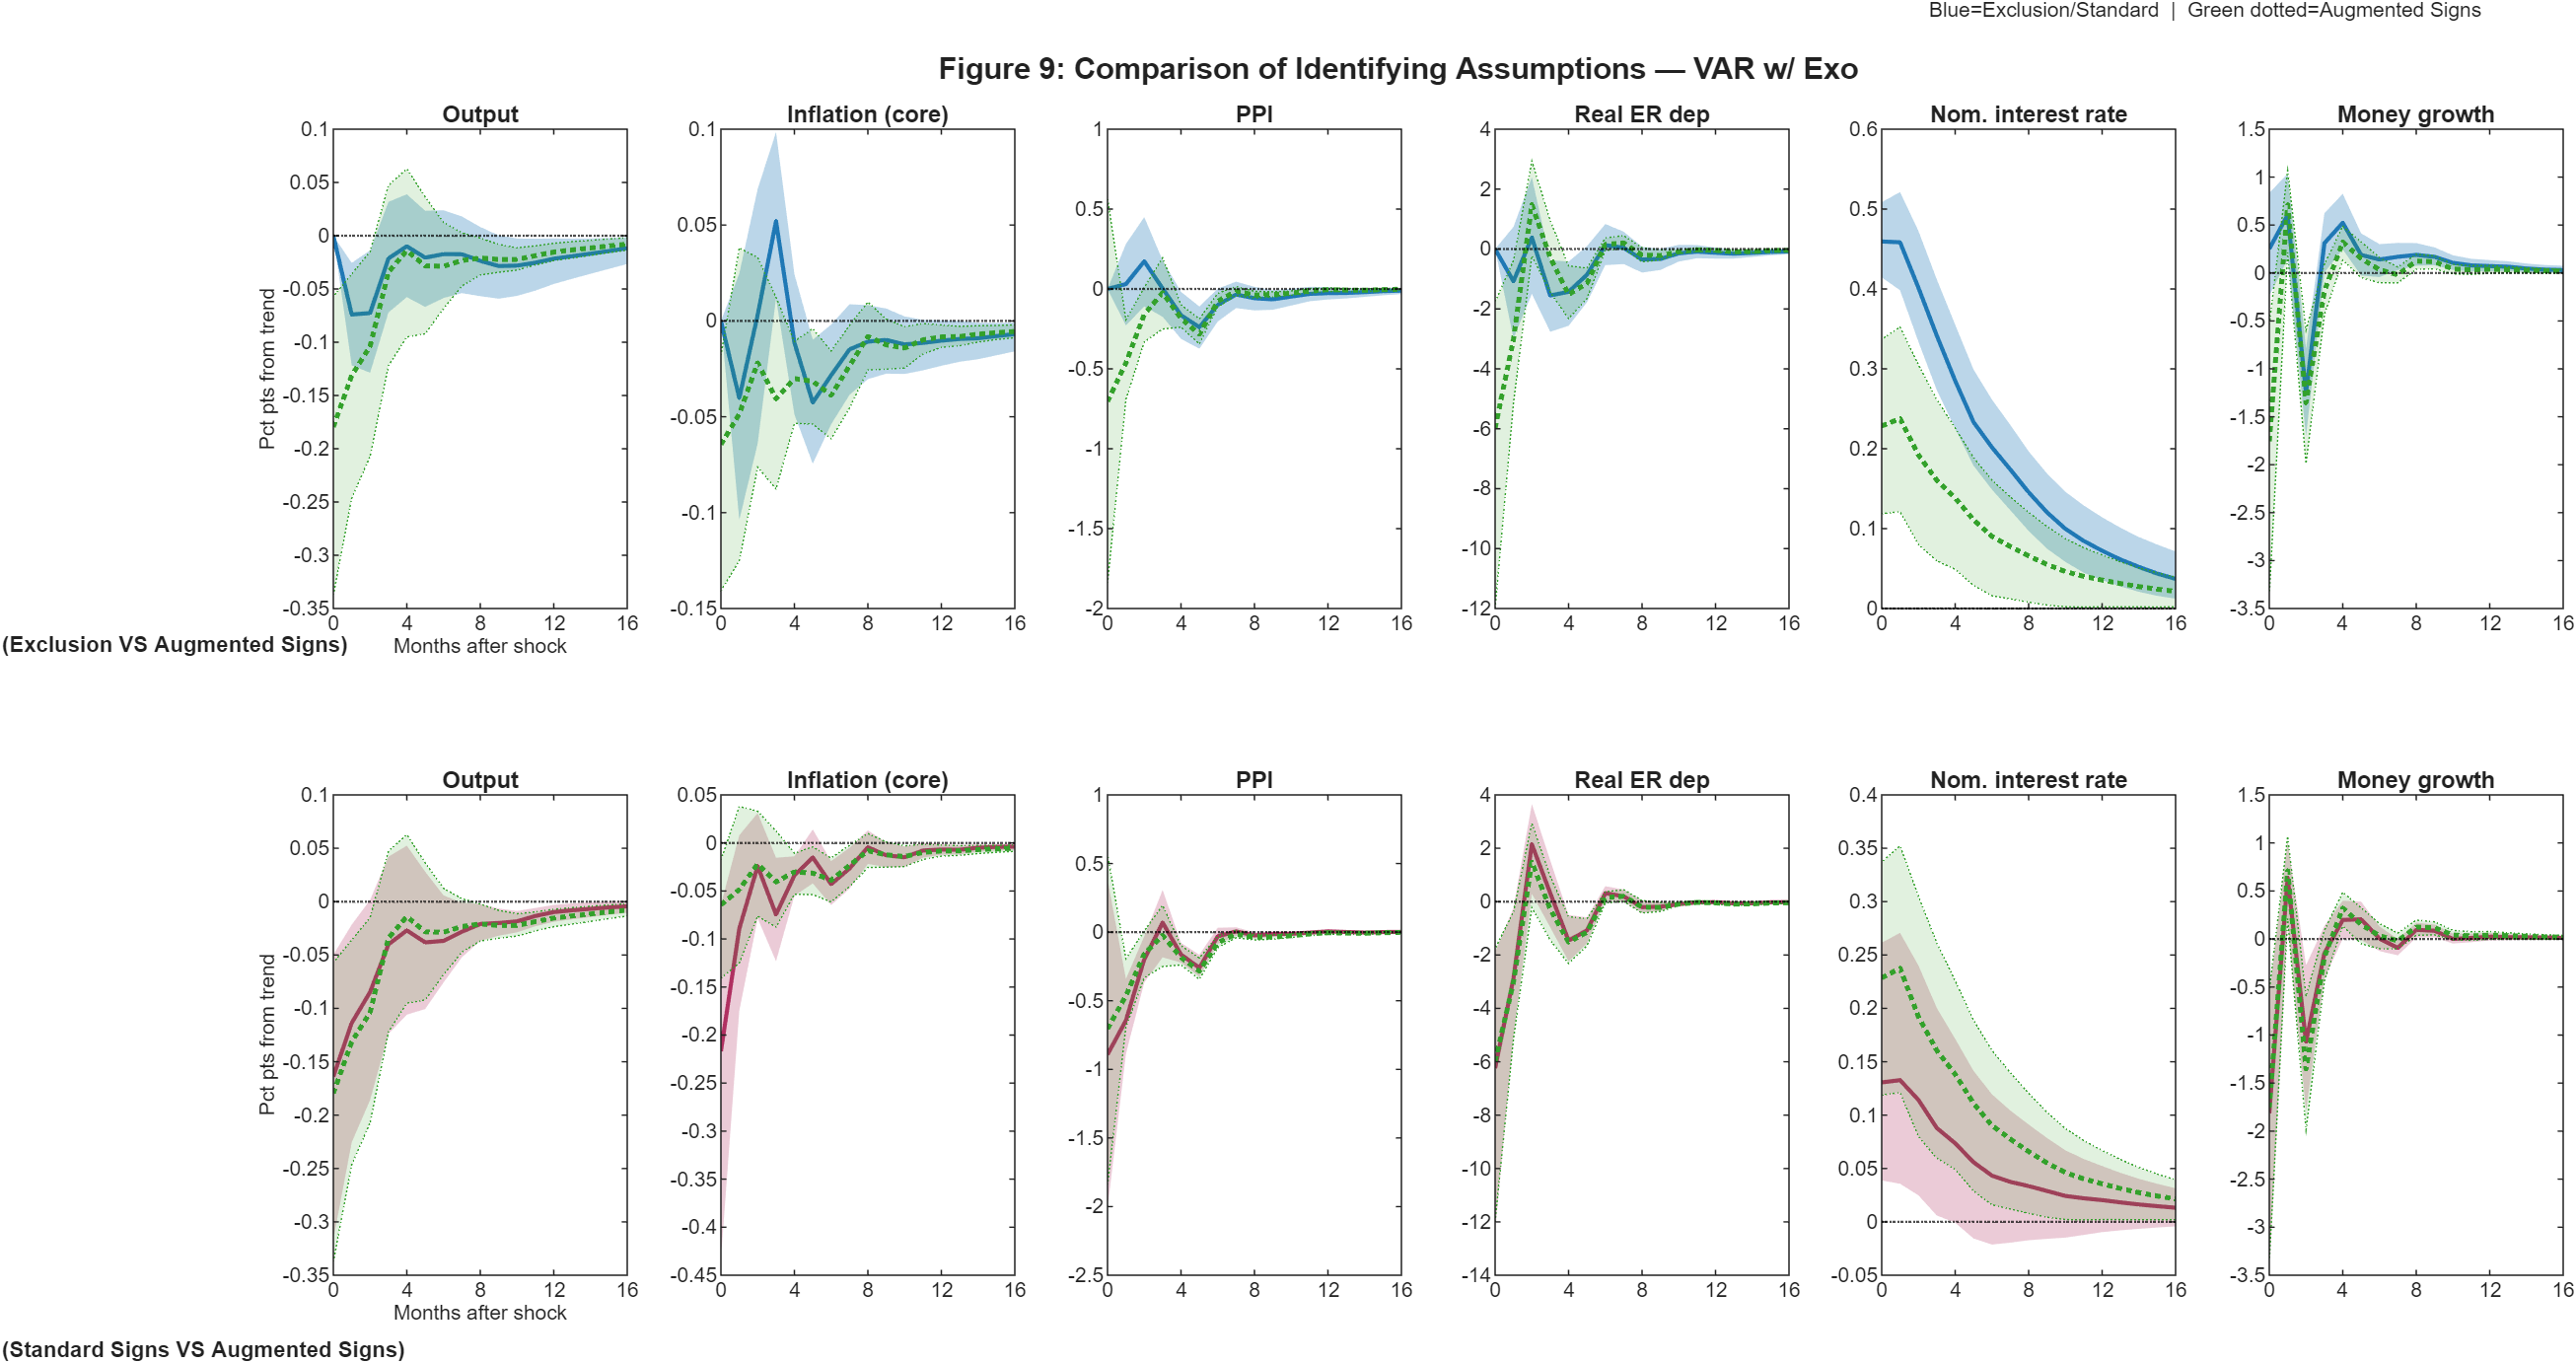
\includegraphics[width=\linewidth,height=0.75\textheight,keepaspectratio]{figures/fig9_comparison.png}
\column{0.40\textwidth}
  \small
  \textbf{Impactos $h=0$ --- 3 estrategias:}
  \vspace{0.15cm}
  \begin{tabular}{lccc}
    \toprule
    Var.       & Chol.   & Std.    & Aug.    \\
    \midrule
    Output     & $0$     & $-0.17$ & $-0.18$ \\
    $\pi$ core & $0$     & $-0.23$ & $-0.06$ \\
    PPI        & $0$     & $-0.95$ & $-0.80$ \\
    TCR        & $0$     & $-6.33$ & $-6.07$ \\
    $i$        & $+0.47$ & $+0.13$ & $+0.23$ \\
    M2         & $+0.31$ & $-1.96$ & $-1.90$ \\
    \bottomrule
  \end{tabular}
  \vspace{0.2cm}
  \small
  \textcolor{green!60!black}{\textbf{Price puzzle eliminado}}
  con restricciones de signo en las tres estrategias.\;\checkmark
\end{columns}
\end{frame}

% =============================================================================
% §4  DIFERENCIAS Y CONCLUSIONES
% =============================================================================

% ── SLIDE 14: TABLA DE DIFERENCIAS ───────────────────────────────────────────
\begin{frame}{\S4 Principales diferencias con el paper}
\small
\renewcommand{\arraystretch}{1.25}
\begin{tabular}{p{2.7cm}p{2.7cm}p{2.7cm}p{3.6cm}}
  \toprule
  \textbf{Dimensi\'on} & \textbf{Paper} & \textbf{Replicaci\'on} & \textbf{Causa probable} \\
  \midrule
  $T$ observaciones
    & 159 & 159
    & \textcolor{green!60!black}{\checkmark} Resuelto: filtro extendido a dic-2000 \\
  TCR bilateral
    & 21 socios & 49 socios
    & Datos disponibles en Banxico \\
  $\hat{\beta}_{lower}$
    & $-0.700$ & $-0.715$
    & Diferencia marginal ($<2\%$) \\
  IRFs Cholesky
    & Fig.~7 paper & Muy similares
    & Bootstrap Runkle completo implementado \\
  Modelos sign rest.
    & N/D en paper & 198,654
    & Sin referencia en el paper \\
  Producto dom\'estico
    & Brecha precalculada & \'Indice IGAE nivel
    & Fuente INEGI directa \\
  \bottomrule
\end{tabular}
\end{frame}

% ── SLIDE 15: CONCLUSIONES ───────────────────────────────────────────────────
\begin{frame}{\S4 Conclusiones}
\begin{itemize}
  \item La replicaci\'on recupera los resultados
        \textbf{cualitativos centrales} del paper de Carrillo \& Elizondo
  \vspace{0.25cm}
  \item \textbf{Price puzzle eliminado} con restricciones de signo
        en las tres estrategias de identificaci\'on
  \vspace{0.25cm}
  \item Diferencia cuantitativa m\'as relevante: TCR
        (49 vs.\ 21 socios) $\Rightarrow$ sin impacto cualitativo en IRFs
  \vspace{0.25cm}
  \item $\hat{\beta}_{lower}$ pr\'acticamente id\'entico:
        $-0.715$ vs.\ $-0.700$
  \vspace{0.25cm}
  \item Restricciones de signo \textbf{aumentadas} operan como
        filtro efectivo sobre la distribuci\'on de modelos aceptados,
        imponiendo consistencia con la elasticidad estimada
        $\hat{\beta}^-=-0.400$
\end{itemize}
\end{frame}

\end{document}
